\chapter{Zeitplan}\label{ch:zeitplan}
Basierend auf den definierten Arbeitspaketen wird ein Zeitplan erstellt, der als Richtwert für die Zehn Tage dient. Die Felder sind in 2-Stunden-Blöcken aufgeteilt. Bei der Arbeit selbst kann aber auf eine Stunde gerundet werden. Aus diesem Grund können auch zwei verschiedene Arbeitspakete auf einer Linie sein. Links am Rand sind die verschiedenen Arbeitspakete beschriftet und haben rechts davon den geschätzten Zeitaufwand (blaue Kästchen), tatsächlichen Zeitaufwand (gelbe Kästchen) und die Differenz.


\begin{figure}[H]
	\begin{center}
		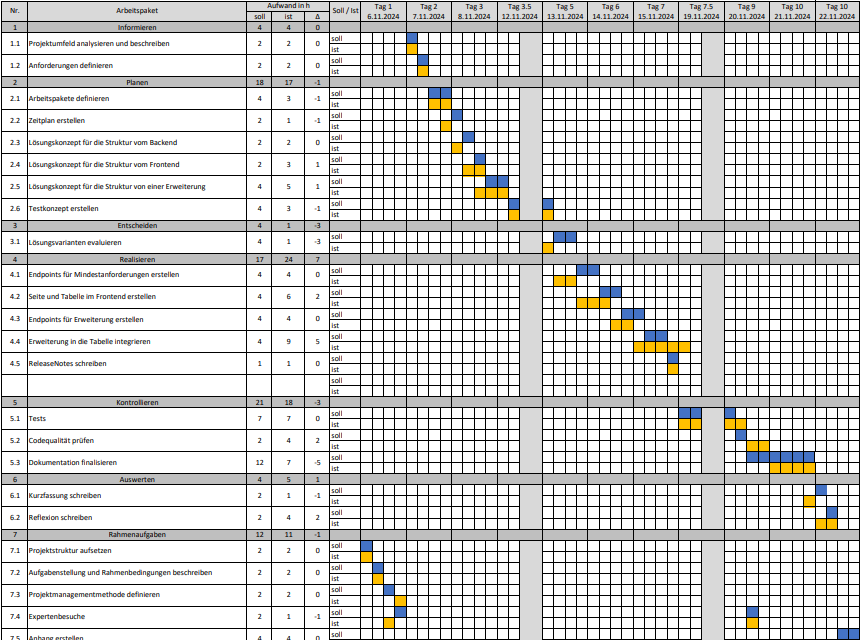
\includegraphics[width=\textwidth]{ressourcen/zeitplan1}
		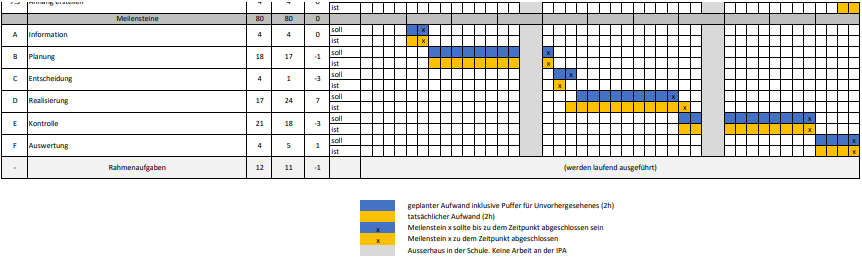
\includegraphics[width=\textwidth]{ressourcen/zeitplan2}
		\caption[Zeitplan]{Zeitplan}\label{fig:zeitplan1}
	\end{center}
\end{figure}

